% Created 2023-05-11 Thu 16:48
% Intended LaTeX compiler: pdflatex
\documentclass[presentation]{beamer}
\usepackage[utf8]{inputenc}
\usepackage[T1]{fontenc}
\usepackage{graphicx}
\usepackage{longtable}
\usepackage{wrapfig}
\usepackage{rotating}
\usepackage[normalem]{ulem}
\usepackage{amsmath}
\usepackage{amssymb}
\usepackage{capt-of}
\usepackage{hyperref}
\usetheme{default}
\usecolortheme{}
\usefonttheme{}
\useinnertheme{}
\useoutertheme{}
\author{Dimitrios Papachistopoulos}
\date{\today}
\title{Investigations of the galaxies of the LCV}

\hypersetup{
 pdfauthor={Dimitrios Papachistopoulos},
 pdftitle={Investigations of the galaxies of the LCV},
 pdfkeywords={},
 pdfsubject={},
 pdfcreator={Emacs 28.2 (Org mode 9.6.1)}, 
 pdflang={English}}
\usepackage{biblatex}
\addbibresource{/home/dp/Documents/Research_paper_SFR/bibl/bibliography/bibliography.bib}
\begin{document}

\maketitle




\begin{frame}[label={sec:org9d0b2d9}]{Abstract}
\begin{block}{LCV}
The paper investigates the properties of galaxies in the Local Cosmological Volume (LCV), using the Catalogue of Neighboring Galaxies\autocite{karachentsevUPDATEDNEARBYGALAXY2013} and its updated version from the ``Catalog \& Atlas of the LV galaxies'' database\autocite{CatalogLVGalaxies}.
\end{block}
\begin{block}{The studied properties}
\begin{enumerate}
\item Galaxy types,
\item Their various masses,
\item The star formation rates (SFRs)
\item Timescales
\begin{enumerate}
\item Star formation timescale \(\tau\),
\item Gas depletion timescale \(\tau_g\)
\item The star formation time \(t_{sf}\).
\end{enumerate}
\end{enumerate}
\end{block}
\begin{block}{Goal}
The paper aims to understand the distribution and correlation of these properties in the sample of galaxies in the LCV, and how they relate to current astrophysical theories.
\end{block}
\end{frame}

\begin{frame}[label={sec:org75f05ef}]{The Galaxies in the Local Cosmological Volume (LCV)}
The Catalogue of Neigbouring Galaxies (Karachentsev, Igor D. and Makarov  et al. 2013\autocite{karachentsevUPDATEDNEARBYGALAXY2013}) and its updated version from the ``Catalog \& Atlas of the LV galaxies'' database\autocite{CatalogLVGalaxies}  are used

\begin{block}{Data}
\begin{enumerate}
\item The B-band, FUV \& K-band luminosities\footnote{We use the FUV and B measurments to calculate the B-FUV color index.} ,
\item The types of the galaxie\footnote{TType=Morphology type code according to the classification by de Vaucouleurs/ Tdw1=Dwarf galaxy morphology/ Tdw2=Dwarf galaxy surface brightness morphology}s,
\item Masses:
\begin{enumerate}
\item The mass within the Holmberg radius (M26)\footnote{\uline{Definition} \alert{Holmberg radius}: \texttt{A convenient measure of the optical extent of a galaxy is the /Holmberg radius/ (Holmberg 1958), which is the major-axis radius at a surface brightness of 26.5 photographic mag arcsec-2}\autocite{MassesMasstoLightRatios}},
\end{enumerate}
\begin{enumerate}
\item The Hydrogen masses of the galaxies (\(M_{HI}\))
\end{enumerate}
\item Their SFRs based on integrated  H and far-ultraviolet (FUV) measurments
\end{enumerate}

\begin{enumerate}
\item The galaxies are within a distance of \(\approx 11\) Mpc.
\item Some of those values contain limit flags, which we exclude from our present analysis. This gives a sample of 793 galaxies from 1248
\end{enumerate}

\begin{center}
\begin{tabular}{|l|l|}
\hline
Measurment & Number of Galaxies \\
\hline
Name & 793 \\
FUVmag & 687 \\
TType & 793 \\
Tdw1 & 580 \\
Tdw2 & 568 \\
Bmag & 790 \\
SFR$\backslash$\_Ha & 566 \\
SFR$\backslash$\_FUV & 688 \\
K & 789 \\
MHI & 643 \\
color & 686 \\
\hline
\end{tabular}
\end{center}

\begin{enumerate}
\item The K-band values are converted to the total Stellar Masses of each galaxy according to the mass-to-light ratio\autocite{lelliSPARCMASSMODELS2016}
$$\frac{M_*}{K}=0.6$$
\item The \(M_{HI}\) can be converted to the total mass of the gas of the galaxy using the equation $$M_g=1.33\cdot M_{HI}$$
\end{enumerate}
\begin{enumerate}
\item The total SFR of each galaxy can be calcuated by
\end{enumerate}

$$
    SFR_o=\frac{SFR_{FUV}+SFR_{Ha}}{2}
$$

$$
    SFR_o=SFR_i,\ \text{if } SFR_j=0,i\neq j,\ i,j=FUV, H_a
$$
\begin{enumerate}
\item We use the FUV and B measurments to calculate the B-FUV color index.
\end{enumerate}

The condition \(SFR_o\geq 10^{-3}M_\odot yr^{-1}\) leaves 579 galaxies. This condition is applied due to the reasons given in the P. Kroupa,M. Haslbauer, I. Banik, S. T. Nagesh and J. Pflamm-Altenburg et al. 2020 \cite{kroupaConstraintsStarFormation2020}
\end{block}
\end{frame}

\begin{frame}[label={sec:org236576b}]{Types of galaxies}
Using the dataset of 1248 galaxies, do before using the condition and removing the galaxies with the flags, the below histograms can be plotted.

\begin{itemize}
\item Most of the galaxies in the LCV are Irregular galaxies followed by lenticular galaxies

\item Out of the 1248 galaxies the 1022 are dwarf galaxies

\item Most dwarf galaxies have low brightness and are irregulars followed by Dwarf spheroidal.
\end{itemize}

\begin{figure}[htbp]
\centering
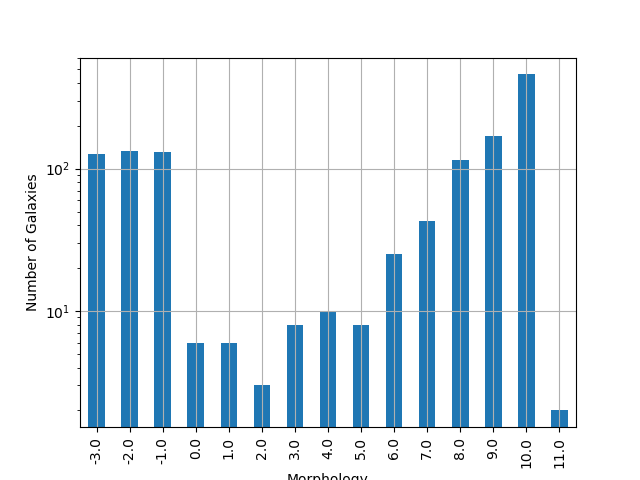
\includegraphics[width=.9\linewidth]{./figs/hist-Type.png}
\caption{\label{Types of galaxies}The classification by de Vaucouleurs et al. (1991) is used for the morphology of the galaxies}
\end{figure}

\begin{figure}[htbp]
\centering
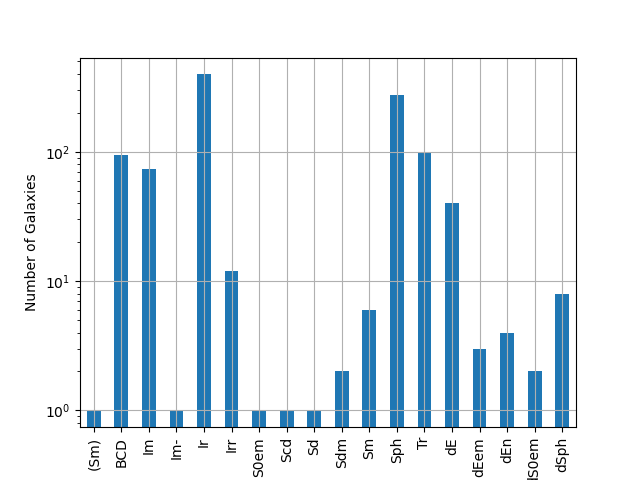
\includegraphics[width=.9\linewidth]{./figs/hist-Tdw1.png}
\caption{\label{Types of dwarf galaxies}Dwarf galaxy morphology}
\end{figure}

\begin{figure}[htbp]
\centering
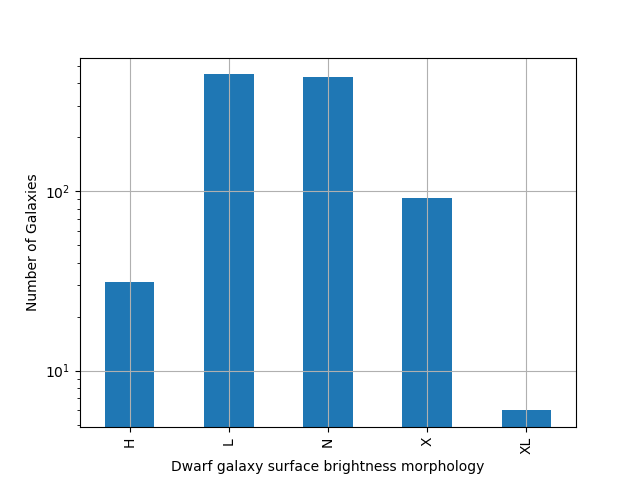
\includegraphics[width=.9\linewidth]{./figs/hist-Tdw2.png}
\caption{\label{Types of dwarf galaxies brightness}Dwarf galaxy surface brightness morphology, where: H = high; N = normal; L = low; X = extremely low.}
\end{figure}
\end{frame}


\begin{frame}[label={sec:org05089e9}]{Delayed-\(\tau\) model}
According to P. Kroupa et al. 2020\autocite{kroupaConstraintsStarFormation2020} current star formation rates of galaxies can be described by the 'delayed-\(\tau\)' model as


\begin{equation} \label{eq:SFR}
SFR_{0,del}=\frac{A_{del}xe^{-x}}{\tau},\text{ where } x=\frac{t_{sf}}{\tau}
\end{equation}

where \(\tau\) is the star formation time-scale,  \(t_{sf}\) is the real time of star formation in a given galaxy and \(A_{del}\) a normalization constant.

The average SFR is

\begin{equation}\label{eq:av_SFR-x}
\overline{SFR_{del}}=\frac{A_{del}}{t_{sf}}[1-(1+x)e^{-x}]
\end{equation}
and can also be defined by the present day stellar mass

\begin{equation}\label{eq:av_SFR M*}
    \overline{SFR}=\frac{\zeta M_*}{t_{sf}}, \zeta = \approx 1.3
\end{equation}

where \(\zeta\) accommodates for mass-loss through stellar evolution

This is a system of 2 equations and 3 variables, since A\textsubscript{del} has never been calculated


\begin{enumerate}
\item Constant \(t_{sf}\)
\item Constant \(\tau\)
\item Integrate the SFR to find the A\textsubscript{del}
\end{enumerate}

\begin{block}{Constant \(t_{sf}\)}
The observed ages of galactic discs are \(t_{sf}\approx 12\) Gyr\autocite{knoxSurveyCoolWhite1999}, so assuming an approximation of \(t_{sf}=12.5\) Gyr, the \(\overline{SFR_{del}}\) can be calcuated, from the equation (\ref{eq:av_SFR M*}).



After that the equation of ratio



\begin{equation} \label{eq:ratio}
    \frac{\overline{SFR_{del}}}{SFR_{0,del}}=\frac{e^x-x-1}{x^2}
\end{equation}

can be solved numerically for \(x\) and using the equations (\ref{eq:SFR}) and (\ref{eq:av_SFR-x}) the \(A_{del}\) and \(\tau\) of each galaxy are found.

\begin{center}
\begin{tabular}{lrrr}
 & A\textsubscript{tsf} & tau & x\textsubscript{tsf}\\[0pt]
\hline
count & 578 & 579 & 579\\[0pt]
mean & 2.24715e+12 & 1.08958e+11 & 1.85344\\[0pt]
std & 3.93675e+13 & 1.04132e+12 & 1.4763\\[0pt]
min & 2.47798e+07 & 1.93205e+09 & 0.000558601\\[0pt]
25\% & 1.40573e+08 & 4.18098e+09 & 0.564779\\[0pt]
50\% & 6.83764e+08 & 7.79265e+09 & 1.60408\\[0pt]
75\% & 5.70379e+09 & 2.21327e+10 & 2.98973\\[0pt]
max & 9.10088e+14 & 2.23774e+13 & 6.46982\\[0pt]
\end{tabular}
\end{center}

\begin{figure}[!htpb]
\centering
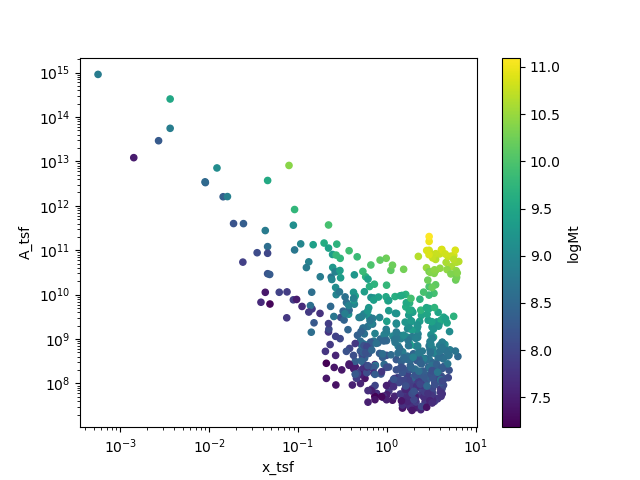
\includegraphics[width=.9\linewidth]{./figs/x-A_tsf.png}
\caption{\label{fig:$A_{del} = f(x)$ for constant t_{sf}}\(A_{del} = f(x)\) for constant t\textsubscript{sf}}
\end{figure}


\begin{figure}[!htpb]
\centering
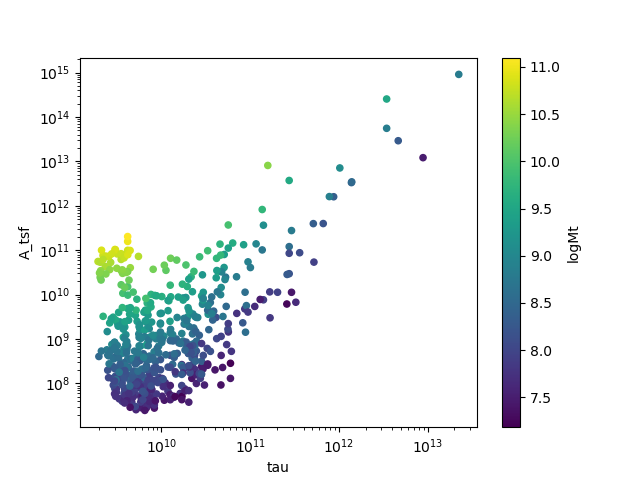
\includegraphics[width=.9\linewidth]{./figs/T-A_tsf.png}
\caption{\label{fig:$A_{del} = f(\tau)$ for constant t_{sf}}\(A_{del} = f(\tau)\) for constant t\textsubscript{sf}}
\end{figure}


\begin{figure}[!htpb]
\centering
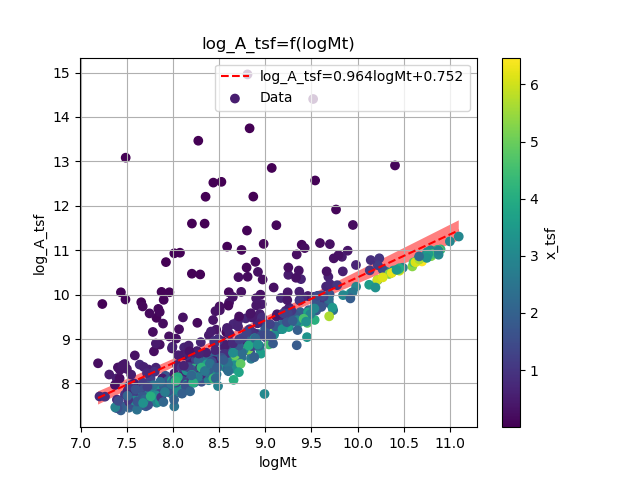
\includegraphics[width=.9\linewidth]{./figs/logMt-log_A_tsf-color_x_tsf.png}
\caption{\label{fig:A_tsf_Mt}Total Mass \(M_t\) - \(A_{del}|_{t_{sf}}\)}
\end{figure}

\begin{equation}\label{eq:logMt-log_A_tsf-color_x_tsf}
\begin{align}
& $log(A_{del}|_t_{sf}) = (9.6(4) \times 10^{-1})\cdot $log(M_t)$ + (8(4) \times 10^{-1}) \\
& \textrm{with correlation } R^2=48\%
\end{align}
\end{equation}
\noindent
\end{block}

\begin{block}{Constant \(\tau\)}
Assuming for an constant \(\tau=3.5\) Gyr, we cannot use the same \(\overline{SFR}\) since it depends on \(t_{sf}\). Using the equations\textasciitilde{}(\Ref{eq:av_SFR M*}) and (\Ref{eq:ratio})

$$
    \frac{\overline{SFR_{del}}}{SFR_{0,del}}=\frac{e^x-x-1}{x^2}\Leftrightarrow \frac{e^x-x-1}{x}=\frac{\zeta M_*}{SFR\cdot\tau}
$$

using this equation \(x\) and \(A_{del}\) can be calculated numerically.




\begin{table}[hc]
\centering
\begin{tabular}{lrrr}
\toprule
{} &    A\_tau &    x\_tau &      tsf \\
\midrule
count & 5.79E+02 & 5.79E+02 & 5.79E+02 \\
mean  & 4.59E+09 & 2.54E+00 & 8.89E+09 \\
std   & 1.50E+10 & 9.57E-01 & 3.35E+09 \\
min   & 9.87E+06 & 4.07E-01 & 1.42E+09 \\
25\%   & 6.50E+07 & 1.87E+00 & 6.55E+09 \\
50\%   & 2.37E+08 & 2.44E+00 & 8.54E+09 \\
75\%   & 1.12E+09 & 3.08E+00 & 1.08E+10 \\
max   & 1.06E+11 & 5.77E+00 & 2.02E+10 \\
\bottomrule
\end{tabular}
\end{table}


\begin{figure}[!htpb]
\centering
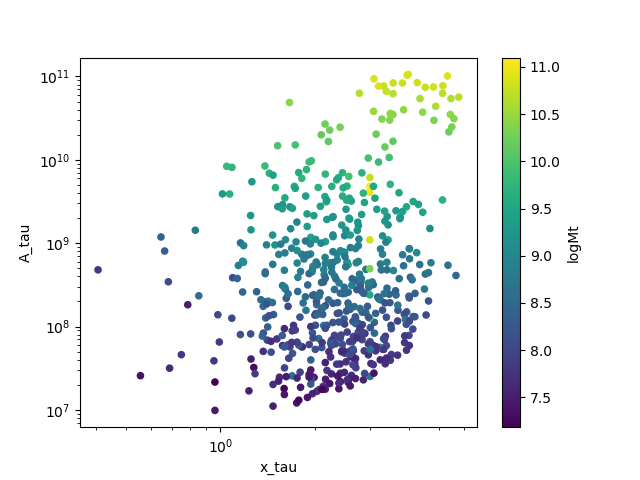
\includegraphics[width=.9\linewidth]{./figs/x-A_tau.png}
\caption{\label{fig:$A_{del} = f(x)$ for constant $\tau$}\(A_{del} = f(x)\) for constant \(\tau\)}
\end{figure}



\begin{figure}[!htpb]
\centering
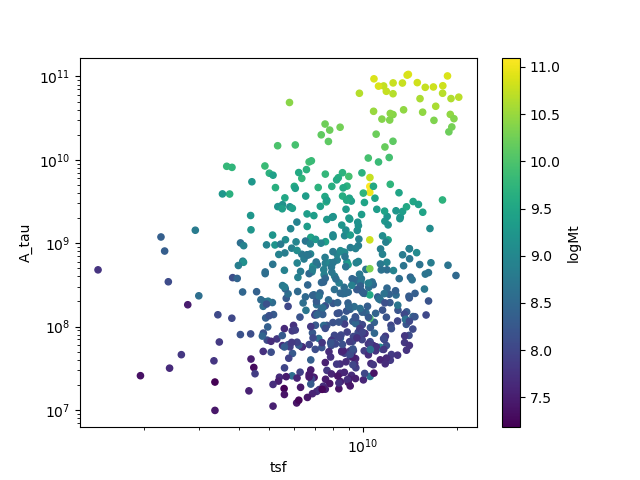
\includegraphics[width=.9\linewidth]{./figs/T-A_tau.png}
\caption{\label{fig:$A_{del} = f(t_{sf})$ for constant $\tau$}\(A_{del} = f(t_{sf})\) for constant \(\tau\)}
\end{figure}


\begin{figure}[!htpb]
\centering
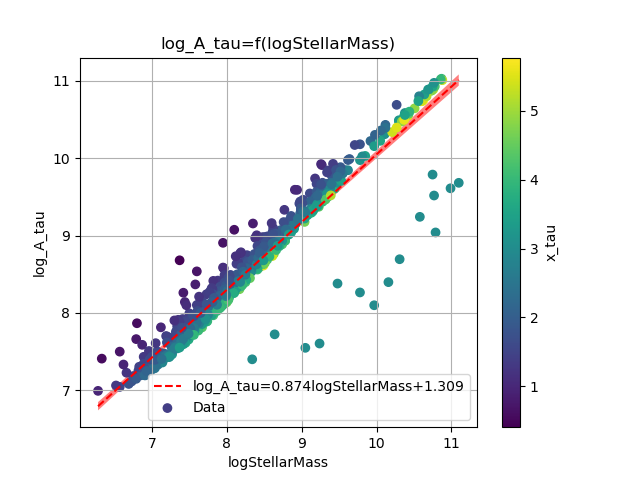
\includegraphics[width=.9\linewidth]{./figs/logStellarMass-log_A_tau-color_x_tau.png}
\caption{\label{fig:A_tau_Mt}Total Mass \(M_t\) - \(A_{del}|_{\tau}\)}
\end{figure}

\begin{equation}\label{eq:logStellarMass-log_A_tau-color_x_tau}
\begin{align}
& $log(A_{del}|_\tau) = (8.74(12) \times 10^{-1})\cdot $log(M_t)$ + (1.31(10) \times 10^{0}) \\
& \textrm{with correlation } R^2=90\%
\end{align}
\end{equation}
\noindent
\end{block}

\begin{block}{Comparing the two results}
\begin{block}{Comparing the \(x\)'s}
Comparing the two different results for x, we see that the \(x|_\tau\) has a lower \(\sigma\)


\begin{table}[hc]
\centering
\begin{tabular}{lrr}
\toprule
{} &    x\_tau &    x\_tsf \\
\midrule
count & 5.79E+02 & 5.79E+02 \\
mean  & 2.54E+00 & 1.85E+00 \\
std   & 9.57E-01 & 1.48E+00 \\
min   & 4.07E-01 & 5.59E-04 \\
25\%   & 1.87E+00 & 5.65E-01 \\
50\%   & 2.44E+00 & 1.60E+00 \\
75\%   & 3.08E+00 & 2.99E+00 \\
max   & 5.77E+00 & 6.47E+00 \\
\bottomrule
\end{tabular}
\end{table}


\begin{figure}[!htpb]
\centering
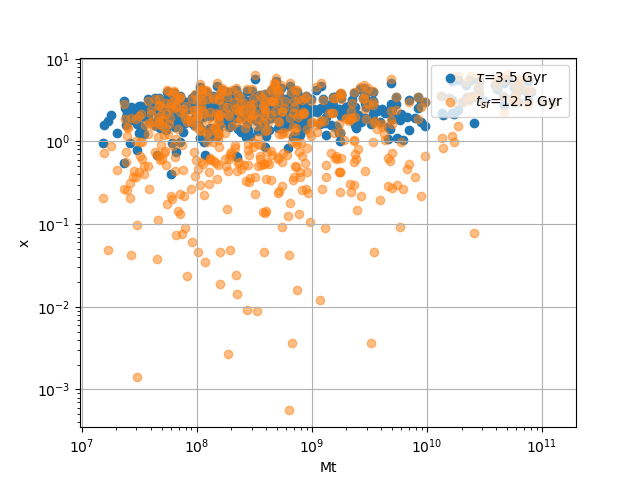
\includegraphics[width=.9\linewidth]{./figs/Comparing_the_x_Mt.png}
\caption{\label{fig:Comparing the two x's, According to their total masses}Comparing the two x's, According to their total masses}
\end{figure}

\begin{figure}[!htpb]
\centering
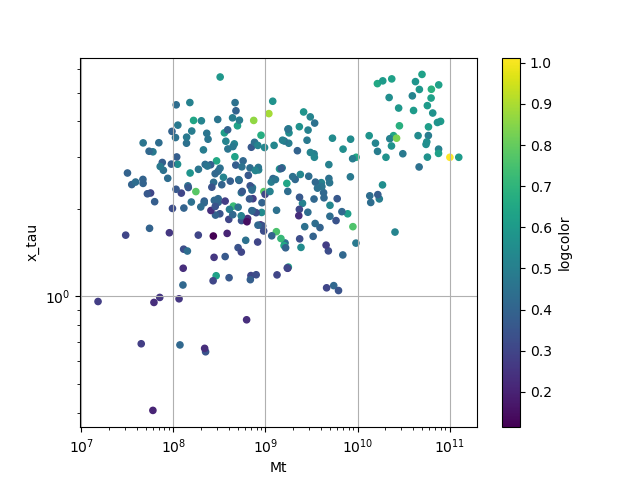
\includegraphics[width=.9\linewidth]{./figs/x_tau-Mt-color.png}
\caption{\label{fig:$x|_\tau=f(M_t)$, with their color index}\(x|_\tau=f(M_t)\), with their color index}
\end{figure}



\begin{figure}[!htpb]
\centering
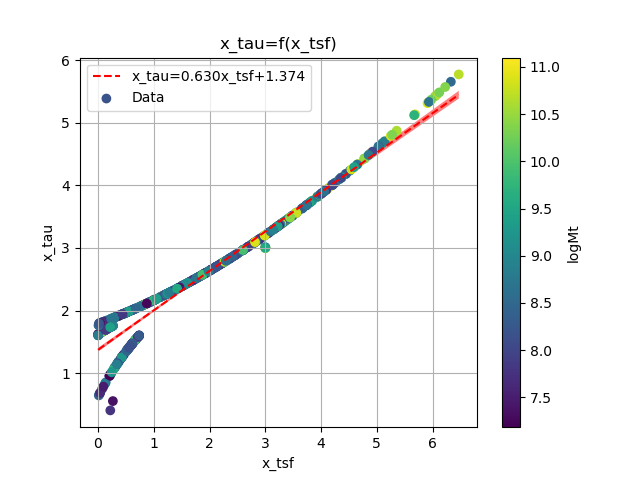
\includegraphics[width=.9\linewidth]{./figs/x_tsf-x_tau-color_logMt.png}
\caption{\label{fig:Comparing the two x, according to their total mass}Comparing the two x, according to their total mass}
\end{figure}


\begin{figure}[!htpb]
\centering
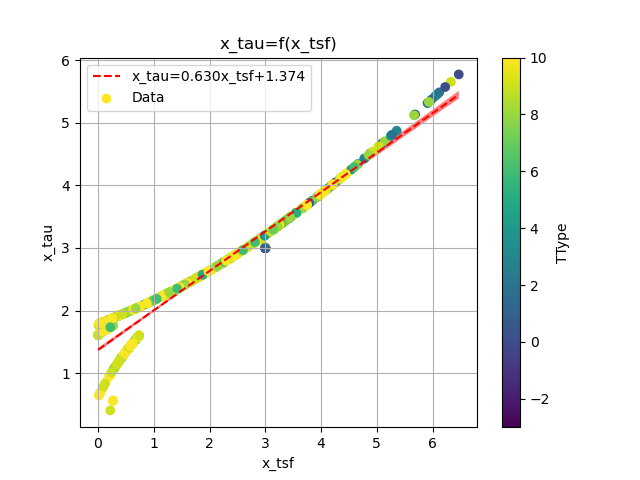
\includegraphics[width=.9\linewidth]{./figs/x_tsf-x_tau-color_TType.png}
\caption{\label{fig:Comparing the two x, according to their type}Comparing the two x, according to their type}
\end{figure}


\begin{figure}[!htpb]
\centering
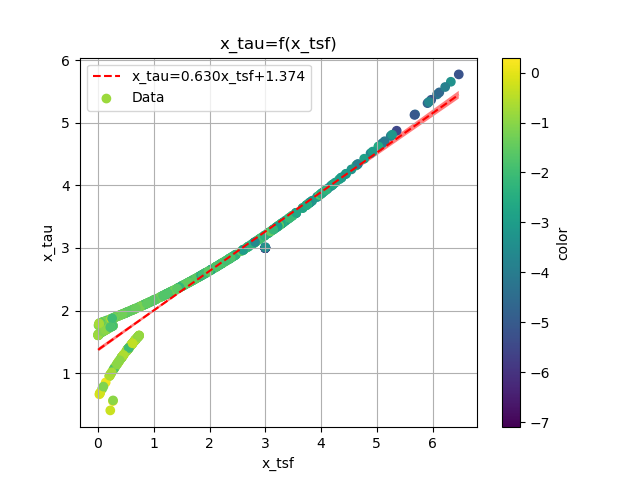
\includegraphics[width=.9\linewidth]{./figs/x_tsf-x_tau-color_color.png}
\caption{\label{fig:Comparing the two x, according to their color index}Comparing the two x, according to their color index}
\end{figure}

The two results are interrelated through the equation:

\begin{equation}\label{eq:x_tsf-x_tau}
\begin{align}
& x|_\tau = (6.30(6) \times 10^{-1})\cdot x|_{tsf} + (1.374(15) \times 10^{0}) \\
& \textrm{with correlation } R^2=94\%
\end{align}
\end{equation}
\noindent

and from the plots the following conclusions can be drawn:

\begin{enumerate}
\item The galaxies with a higher total mass deviate less from the linear fit and are older.
\item The younger galaxies are mainly later types of galaxies
\item For lower x's, the galaxies have a lower color index which indicates that they are younger. So the values are inline with the experimental values.
\end{enumerate}
\end{block}

\begin{block}{Comparing the normalization constants}
\begin{figure}[!htpb]
\centering
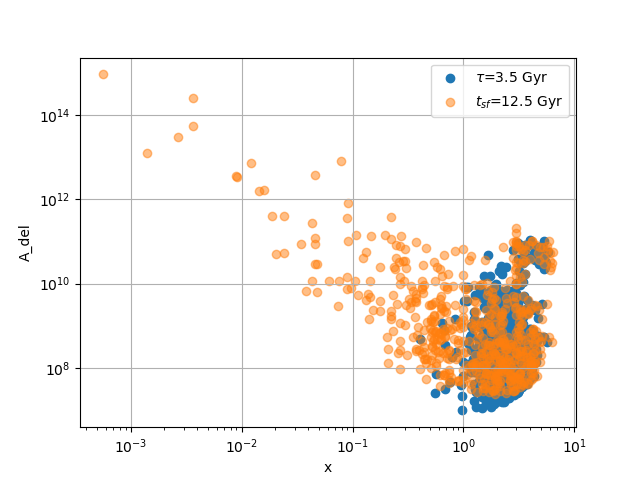
\includegraphics[width=.9\linewidth]{./figs/Comparing_the_A_x.png}
\caption{\label{fig:Comparing the two A_{del}}Comparing the two A\textsubscript{del}}
\end{figure}



\begin{figure}[!htpb]
\centering
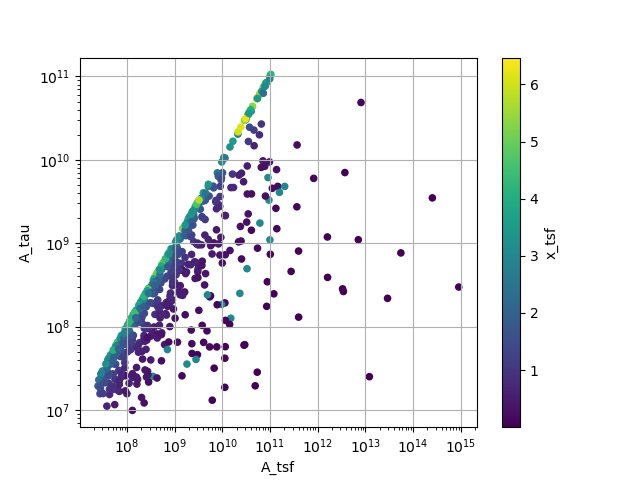
\includegraphics[width=.9\linewidth]{./figs/A_tau-A_tsf_colo_X.png}
\caption{\label{fig:Comparison of the 2 A_{del}s according to their $x$}Comparison of the 2 A\textsubscript{del}s according to their \(x\)}
\end{figure}

\begin{figure}[!htpb]
\centering
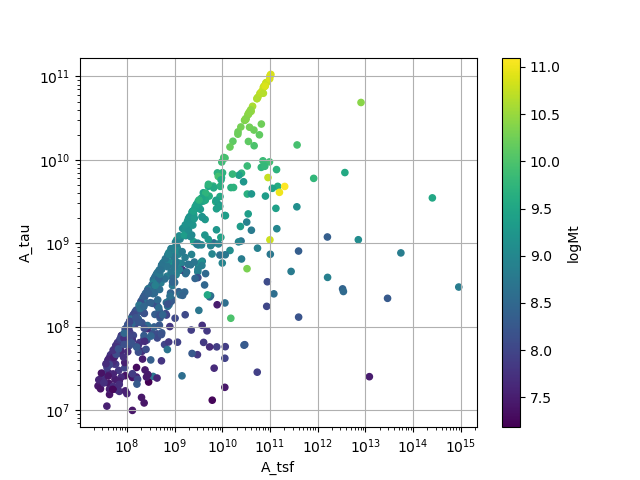
\includegraphics[width=.9\linewidth]{./figs/A_tau-A_tsf_Mt.png}
\caption{\label{fig:Comparison of the 2 A_{del}s according to their total masses}Comparison of the 2 A\textsubscript{del}s according to their total masses}
\end{figure}

For high \(x\) and high masses the two A\textsubscript{del}s have a high correlation. Specifically:
\begin{enumerate}
\item For high \(x\) the \(A_{del}|_{\tau}-A_{del}|_{t_{sf}}\) plot follows a \(y=x\) trend, which means that for older stars and stars with a low star formation timescale \(\tau\), the normalization constant is the same despite the method used to calculate it.
\item The same is true for more massive galaxies, since they deviate less from the \(y=x\) line
\end{enumerate}
\end{block}

\begin{block}{Trying to make the A\textsubscript{del} cloud more compact}
Having found \(x|_{t_sf}\) and \(x|_{\tau}\) we can find a relation between these two values


\begin{figure}[!htpb]
\centering
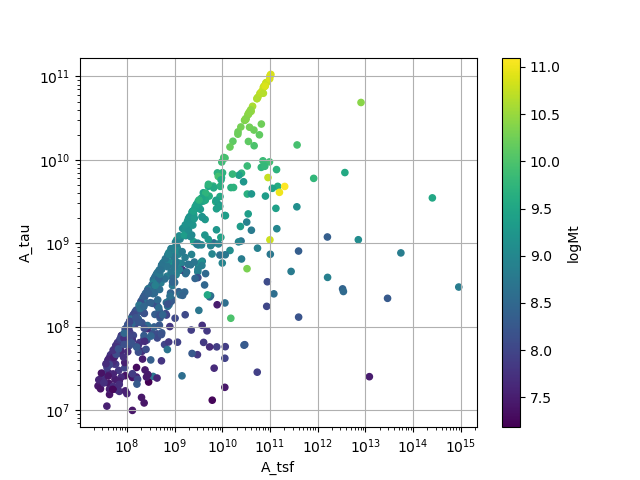
\includegraphics[width=.9\linewidth]{./figs/A_tau-A_tsf_Mt.png}
\caption{\label{fig:Comparison of the 2 A_{del}s according to their total masses}Comparison of the 2 A\textsubscript{del}s according to their total masses}
\end{figure}
\end{block}
\end{block}


\begin{block}{Int SFR to find the A\textsubscript{del}}
If we integrate equation (\ref{eq:SFR}) we get:


\begin{equation}\label{eq:int SFR}
\begin{align}
\int^{t_{sf}}_0 SFR_{del} dt_{sf}&=\int^{t_{sf}}_0 \frac{A_{del}t_{sf}e^{-t_{sf}/\tau}}{\tau^2} dt_{sf}\\
M_*&=-A_{del} \frac{{\left(t_{\mathit{sf}} \tau + \tau^{2}\right)} e^{\left(-\frac{t_{\mathit{sf}}}{\tau}\right)}}{\tau^{2}}+A_{del}\\
M_*&=-A_{del}\frac{\tau^2(x+1)e^{-x}}{\tau^2}+A_{del}\\
M_*& = A_{del}(1-(x+1)e^{-x})\\
A_{del}&=M_*\frac{e^x}{e^x-x-1}
\end{align}
\end{equation}


\begin{figure}[!htpb]
\centering
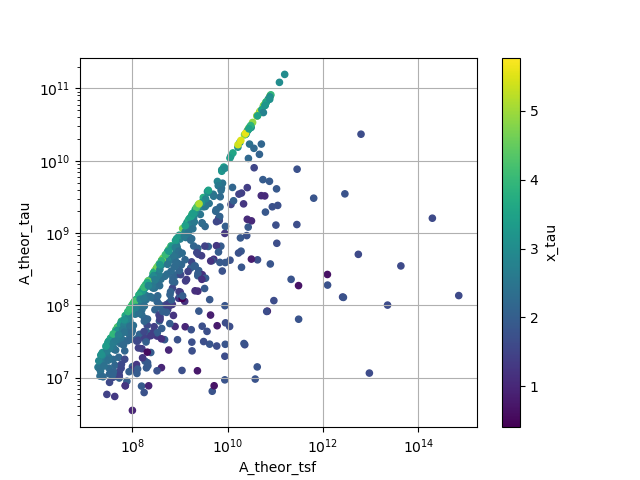
\includegraphics[width=.9\linewidth]{./figs/A_theor_tau-M*.png}
\caption{\label{fig:Comparison of the 2 A_{del}s according to their total masses}Comparison of the 2 A\textsubscript{del}s according to their total masses}
\end{figure}


\begin{figure}[!htpb]
\centering
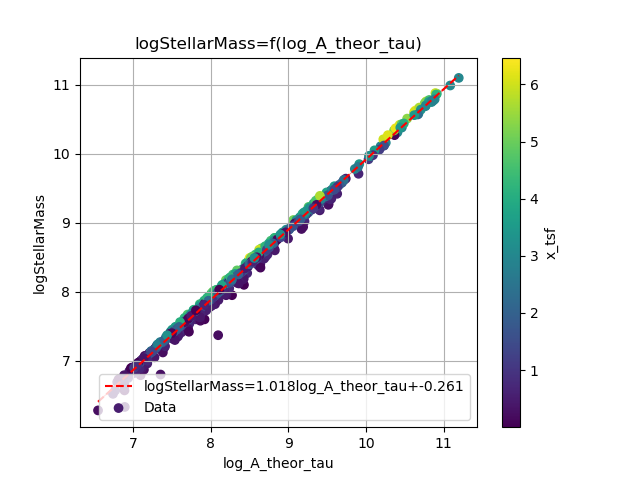
\includegraphics[width=.9\linewidth]{./figs/log_A_theor_tau-logStellarMass-color_x_tsf.png}
\caption{\label{fig:Comparison of the A_del according to their Stellar Mass}Comparison of the A\textsubscript{del} according to their Stellar Mass}
\end{figure}
\end{block}
\end{frame}



\begin{frame}[label={sec:org40e1c03}]{The gas depletion timescale \(\tau_g\) \label{SEC:tau_g}}
The gas depletion timescale \(\tau_g\) measures the time taken by a galaxy to exhaust its gas content Mg given the current SFR\autocites{nageshSimulationsStarformingMainsequence2023}[][]{pflamm-altenburgFundamentalGasDepletion2009}.
\begin{equation}\label{eq:tau_g}
\tau_g=\frac{M_g}{\dot{M_*}}=\frac{M_g}{SFR}
\end{equation}




\begin{center}
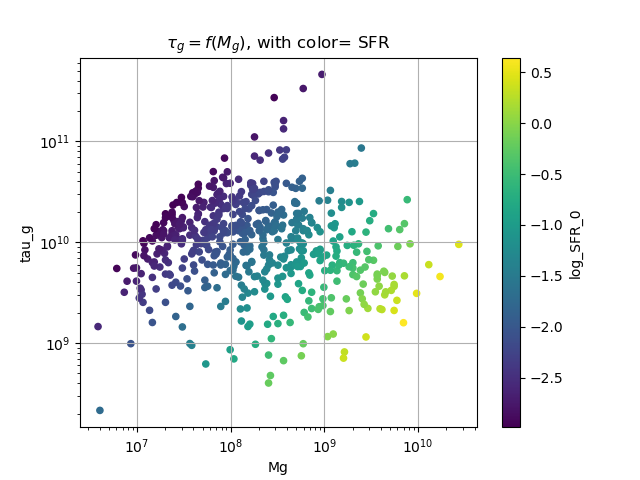
\includegraphics[width=.9\linewidth]{./figs/tau_g-Mg-color_SFR.png}
\end{center}
\begin{figure}[!htpb]
\centering
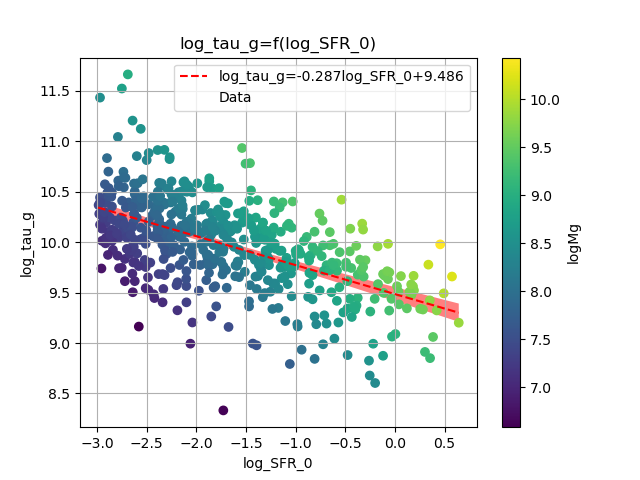
\includegraphics[width=.9\linewidth]{./figs/log_SFR_0-log_tau_g-color_logMg.png}
\caption{\label{fig:Correlation of the $\tau_g$ with the SFR and the gas mass}Correlation of the \(\tau_g\) with the SFR and the gas mass}
\end{figure}

Despite a weak logarithmic correlation (as indicated by ==), there is a noticeable trend of decreasing \(\tau_g\) with increasing SFR and \(M_g\).


\begin{figure}[!htpb]
\centering
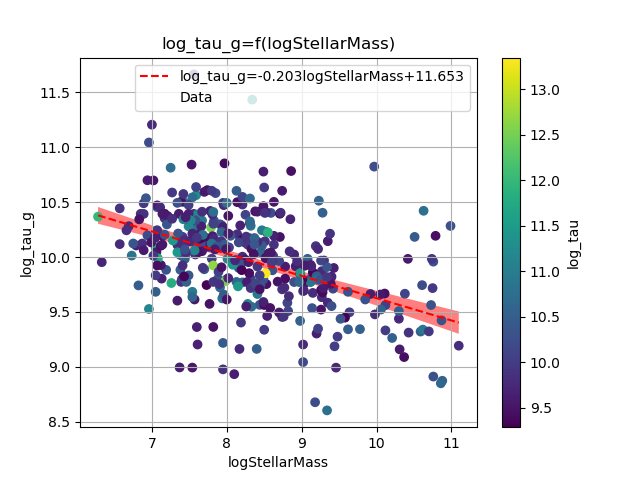
\includegraphics[width=.9\linewidth]{./figs/logStellarMass-log_tau_g-color_log_tau.png}
\caption{\label{fig:Correlation of the $\tau_g$ with the SFR and the Stellar mass}Correlation of the \(\tau_g\) with the SFR and the Stellar mass}
\end{figure}

The logarithmic correlation between \(\tau_g-M_*\) is low (==), there seems to be a pattern wherein the decrease of \(\tau_g\) corresponds to an increase in the values of the Stellar Mass, but there does not seem to be one for \(\tau_g-\tau\)


\begin{figure}[!htpb]
\centering
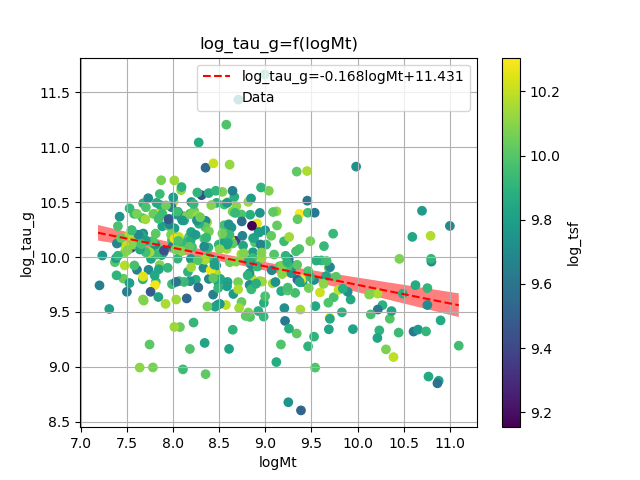
\includegraphics[width=.9\linewidth]{./figs/logMt-log_tau_g-color_log_tsf.png}
\caption{\label{fig:Correlation of the $\tau_g$ with the total mass and the mass of the gas}Correlation of the \(\tau_g\) with the total mass and the mass of the gas}
\end{figure}


\begin{figure}[!htpb]
\centering
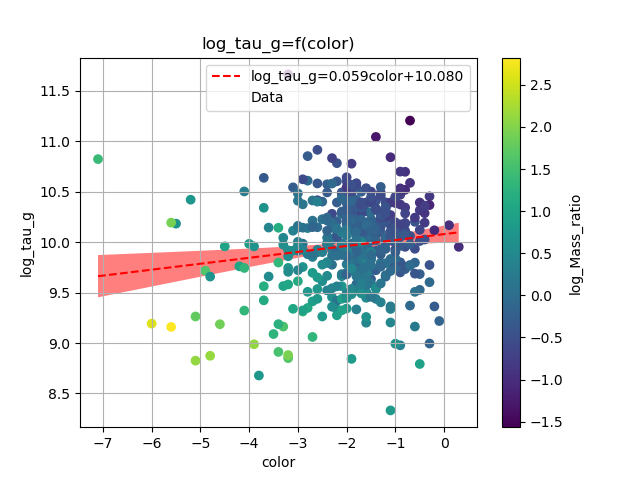
\includegraphics[width=.9\linewidth]{./figs/color-log_tau_g-color_log_Mass_ratio.png}
\caption{\label{fig:Correlation of the $\tau_g$ with the color index}Correlation of the \(\tau_g\) with the color index}
\end{figure}


\begin{figure}[!htpb]
\centering
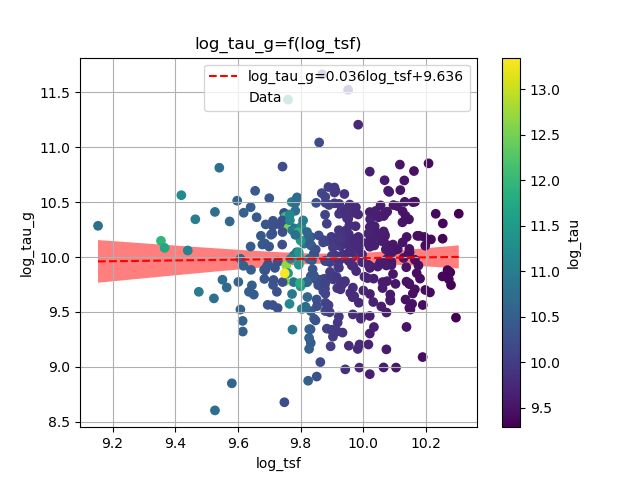
\includegraphics[width=.9\linewidth]{./figs/log_tsf-log_tau_g-color_log_tau.png}
\caption{\label{fig:Correlation of the $\tau_g$ with the color index}Correlation of the \(\tau_g\) with the color index}
\end{figure}

Again it can be observed that as the \(\tau_g\) decreases, the corresponding values of \(M_t\) increase, but the logarithmic correlation is again low (==), and there is no clear correlation between \(\tau_g-t_{sf}\)

There is a notable trend, wherein for high masses we have a shorter timescale.
\end{frame}

\begin{frame}[label={sec:orgfa6d8ce}]{Mass relations}
Many of the galaxies masses have a high correlation with each other, and also help us understand the previous calculations.




\begin{figure}[!htpb]
\centering
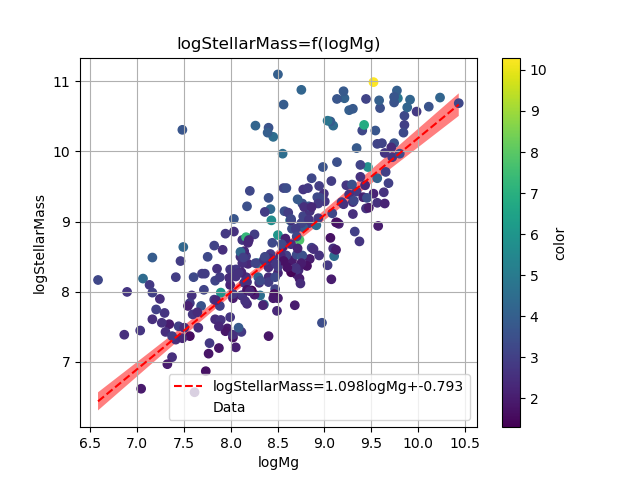
\includegraphics[width=.9\linewidth]{./figs/logMg-logStellarMass-color_color.png}
\caption{\label{fig:mg_SMass}Gas Mass-Stellar Mass plot}
\end{figure}

For the plot \ref{fig:mg_SMass}:

\begin{equation}\label{eq:logMg-logStellarMass}
\begin{align}
& $M_g$ = (1.098(35) \times 10^{0})\cdot $M_*$ + (-7.9(2.9) \times 10^{-1}) \\
& \textrm{with correlation } R^2=64\%
\end{align}
\end{equation}
\noindent


\begin{figure}[!htpb]
\centering
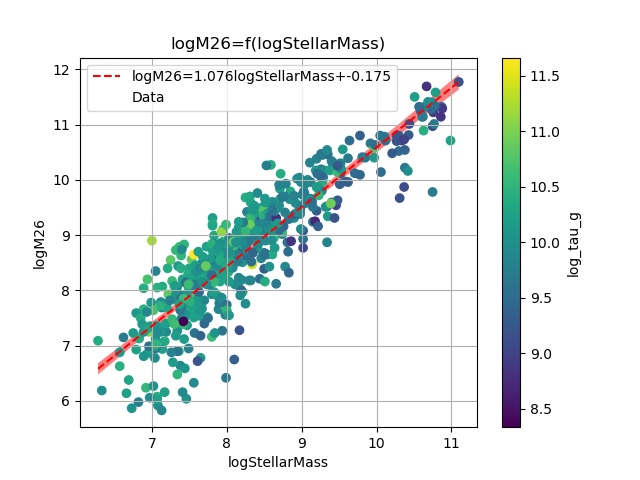
\includegraphics[width=.9\linewidth]{./figs/logStellarMass-logM26-color_log_tau_g.png}
\caption{\label{fig:SMass_m26}Mass inside the Holmberg radius-Stellar Mass plot}
\end{figure}

For the plot \ref{fig:SMass_m26}:


\begin{equation}\label{eq:logStellarMass-logM26}
\begin{align}
& M26 = (1.076(23) \times 10^{0})\cdot M* + (-1.8(1.9) \times 10^{-1}) \\
& \textrm{with correlation } R^2=80\%
\end{align}
\end{equation}
\noindent


\begin{figure}[!htpb]
\centering
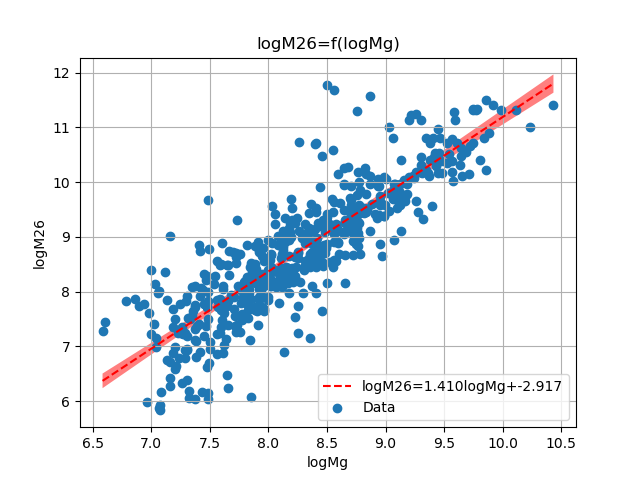
\includegraphics[width=.9\linewidth]{./figs/logMg-logM26.png}
\caption{\label{fig:mg_m26}Mass inside the Holmberg radius-Gas Mass plot}
\end{figure}

For the plot \ref{fig:mg_m26}:


\begin{equation}\label{eq:logMg-logM26}
\begin{align}
& M26 = (1.41(4) \times 10^{0})\cdot Mg + (-2.92(30) \times 10^{0}) \\
& \textrm{with correlation } R^2=74\%
\end{align}
\end{equation}
\noindent


\begin{figure}[!htpb]
\centering
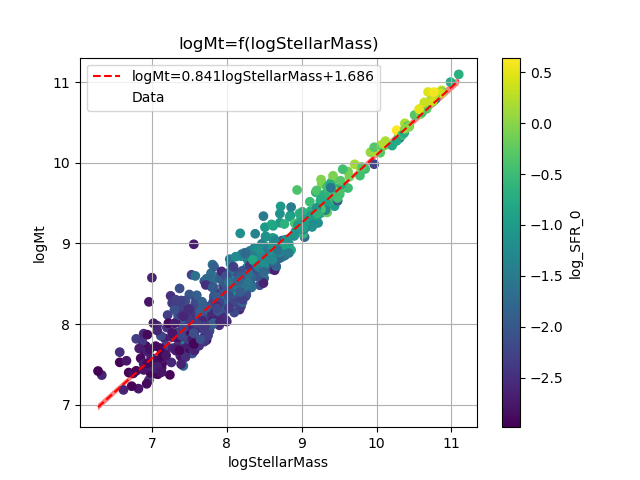
\includegraphics[width=.9\linewidth]{./figs/logStellarMass-logMt-color_log_SFR_0.png}
\caption{\label{fig:SMass_mt}Stellar Mass-Total Mass plot}
\end{figure}

For the plot \ref{fig:SMass_mt}:

\begin{equation}\label{eq:logStellarMass-logMt}
\begin{align}
& $M_t$ = (8.41(9) \times 10^{-1})\cdot $M_*$ + (1.69(8) \times 10^{0}) \\
& \textrm{with correlation } R^2=94\%
\end{align}
\end{equation}
\noindent



\begin{figure}[!htpb]
\centering
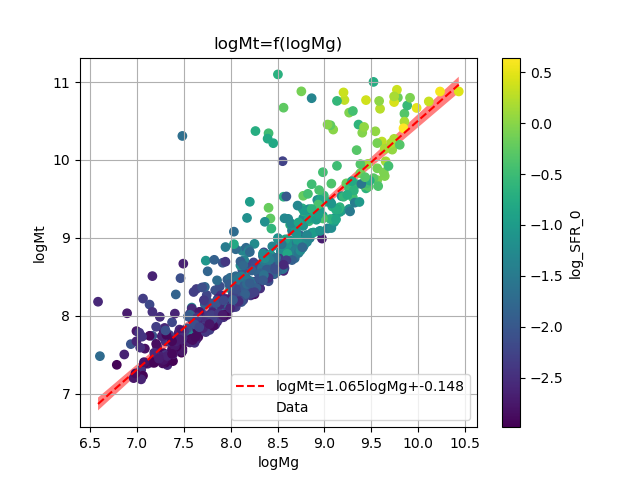
\includegraphics[width=.9\linewidth]{./figs/logMg-logMt-color_log_SFR_0.png}
\caption{\label{fig:mg_mt}Total Mass - Gas Mass plot}
\end{figure}

For the plot \ref{fig:mg_mt}:

\begin{equation}\label{eq:logMg-logMt-color_log_SFR_0}
\begin{align}
& $M_t$ = (1.065(23) \times 10^{0})\cdot $M_g$ + (-1.5(1.9) \times 10^{-1}) \\
& \textrm{with correlation } R^2=81\%
\end{align}
\end{equation}
\noindent



\begin{figure}[!htpb]
\centering
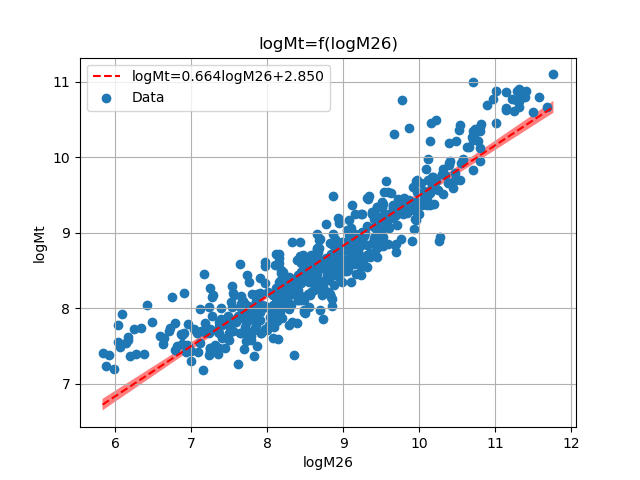
\includegraphics[width=.9\linewidth]{./figs/logM26-logMt.png}
\caption{\label{fig:m26_mt}Mass inside the Holmberg radius-Total Mass plot}
\end{figure}


\begin{equation}\label{eq:logM26-logMt}
\begin{align}
& M26 = (6.64(12) \times 10^{-1})\cdot $M_t$ + (2.85(11) \times 10^{0}) \\
& \textrm{with correlation } R^2=85\%
\end{align}
\end{equation}
\noindent


There are many plots exhibiting a correlation of \(R^2>80%\), indicating that we can utilize those functions to estimate the masses of the galaxies in the LCV with a high degree of confidence.

The \(M_t-M_*\) (\ref{fig:SMass_mt}) plot is particularly noteworthy, displaying a correlation  of ==. This plot also indicates that galaxies with greater total and stellar masses tend to have higher SFR, consistent with the findings in section \ref{SEC:tau_g} where \(\tau_g\) decreases with increasing masses.

This phenomenon is likely due to the fact that galaxies with higher masses possess greater potential energy, which accelerates the star formation process. The galaxies with a high Mass ratio \(M_r\) could also help the process due to their dense regions and the resulting strong local gravitational potential.



\begin{figure}[!htpb]
\centering
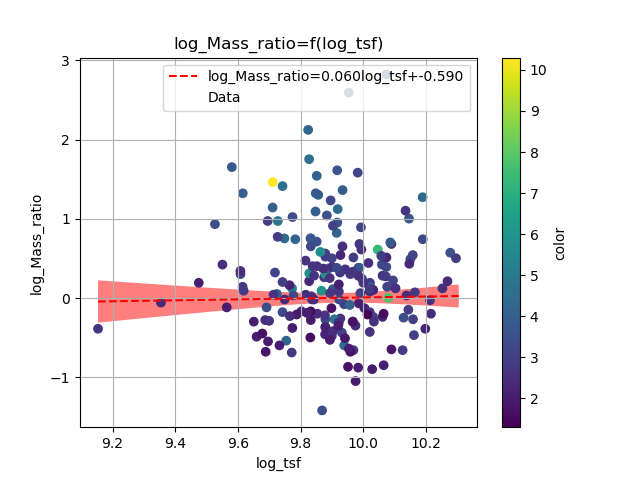
\includegraphics[width=.9\linewidth]{./figs/log_tsf-log_Mass_ratio-color_color.png}
\caption{\label{fig:tsf_mr}\$\t\textsubscript{sf}\$-Mass ratio \(\left(\frac{M_*}{M_g}\right)\) plot}
\end{figure}



\begin{figure}[!htpb]
\centering
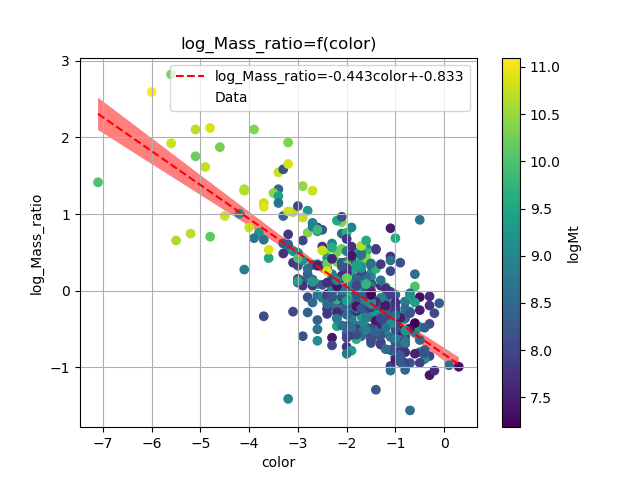
\includegraphics[width=.9\linewidth]{./figs/color-log_Mass_ratio-color_logMt.png}
\caption{\label{fig:col_Mr}Mass ratio \$\frac{M_*}{M_g}\$-Color index plot}
\end{figure}

From the \ref{fig:col_Mr}, we conclude that when the color index is higher the Mass ratio decreases, which is to be expected, since the higher the B-FUV the more active the star formation of the galaxy.
\end{frame}



\begin{frame}[label={sec:orgbd7dd9c}]{Variations in Star Formation Rate Across the Different Masses}
\begin{figure}[!htpb]
\centering
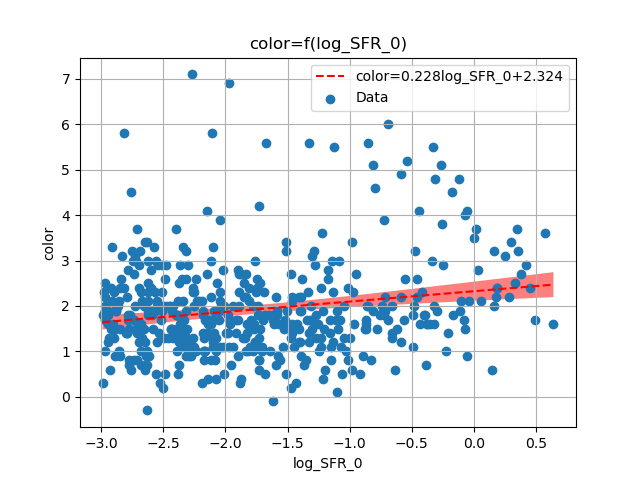
\includegraphics[width=.9\linewidth]{./figs/log_SFR_0-color.png}
\caption{\label{fig:None}None}
\end{figure}


\begin{figure}[!htpb]
\centering
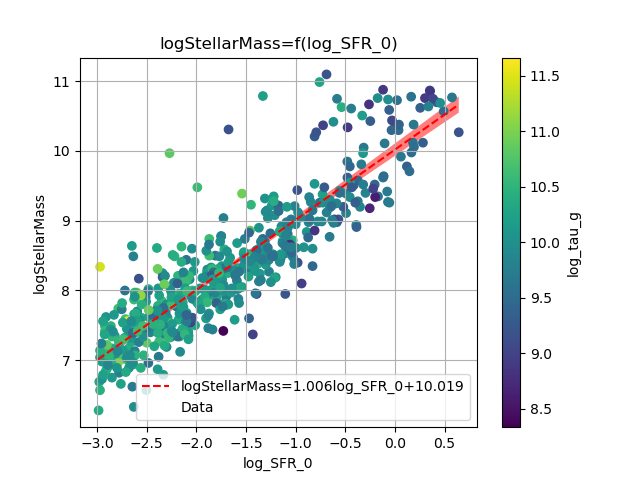
\includegraphics[width=.9\linewidth]{./figs/log_SFR_0-logStellarMass-color_log_tau_g.png}
\caption{\label{fig:None}None}
\end{figure}



\begin{figure}[!htpb]
\centering
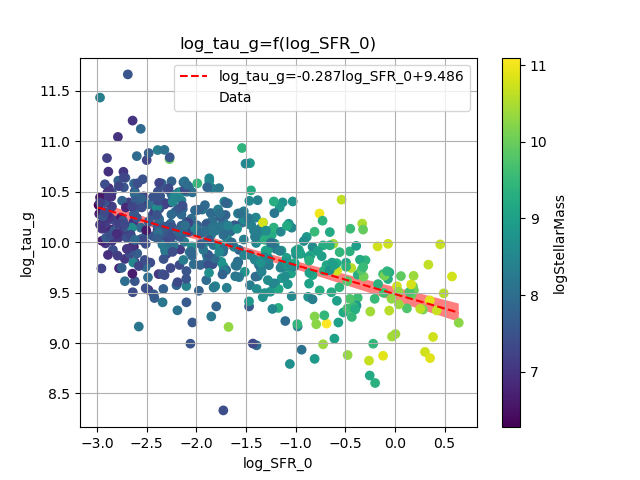
\includegraphics[width=.9\linewidth]{./figs/log_SFR_0-log_tau_g-color_logStellarMass.png}
\caption{\label{fig:None}None}
\end{figure}

\begin{figure}[!htpb]
\centering
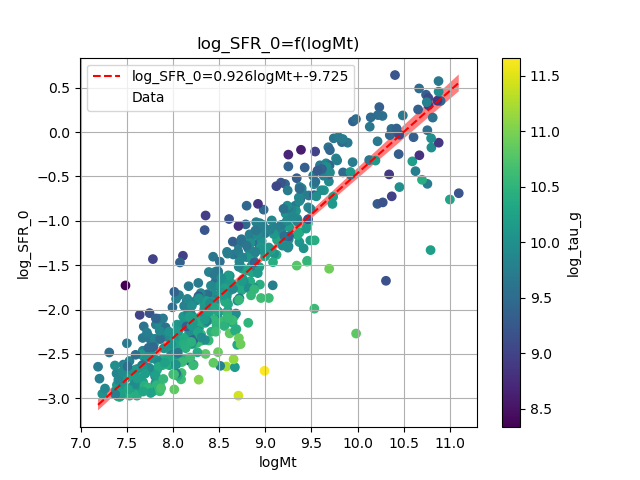
\includegraphics[width=.9\linewidth]{./figs/logMt-log_SFR_0-color_log_tau_g.png}
\caption{\label{fig:None}None}
\end{figure}

\begin{figure}[!htpb]
\centering
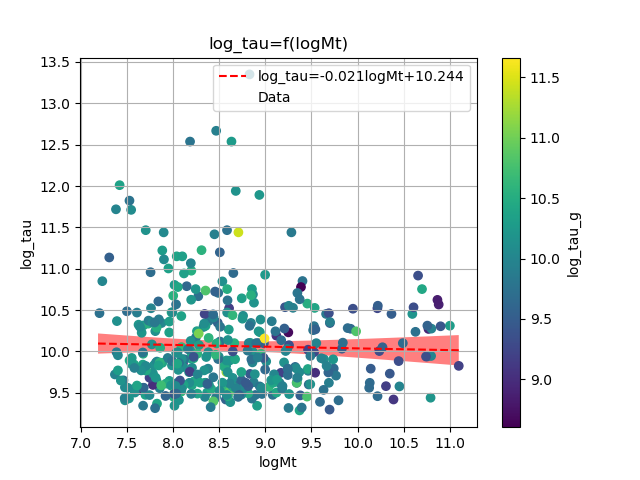
\includegraphics[width=.9\linewidth]{./figs/logMt-log_tau-color_log_tau_g.png}
\caption{\label{fig:None}None}
\end{figure}'

\begin{block}{put that tau and tsf dont have a correlation with Mt}
\pagebreak
\printbibliography
\end{block}
\end{frame}
\end{document}